% This must be in the first 5 lines to tell arXiv to use pdfLaTeX, which is strongly recommended.
\pdfoutput=1
% In particular, the hyperref package requires pdfLaTeX to break URLs across lines.

\documentclass[11pt]{article}

% Remove the "review" option to generate the final version.
\usepackage{NLPAICS2024}

% Standard package includes
\usepackage{times}
\usepackage{latexsym}

% For proper rendering and hyphenation of words containing Latin characters (including in bib files)
\usepackage[T1]{fontenc}
% For Vietnamese characters
% \usepackage[T5]{fontenc}
% See https://www.latex-project.org/help/documentation/encguide.pdf for other character sets

% This assumes your files are encoded as UTF8
\usepackage[utf8]{inputenc}

% This is not strictly necessary, and may be commented out.
% However, it will improve the layout of the manuscript,
% and will typically save some space.
\usepackage{microtype}

% This is also not strictly necessary, and may be commented out.
% However, it will improve the aesthetics of text in
% the typewriter font.
\usepackage{inconsolata}

% Include todo notes
\usepackage{todonotes}

\usepackage{enumitem}

\usepackage{xspace}

\newcommand{\gptthree}{GPT-3.5-turbo\xspace}
\newcommand{\gptfour}{GPT-4-turbo\xspace}
\newcommand{\falconlong}{Falcon-7b-instruct\xspace}
\newcommand{\falcon}{Falcon-7b\xspace}
\newcommand{\gemmalong}{Gemma-7b-it\xspace}
\newcommand{\gemma}{Gemma-7b\xspace}
\newcommand{\mistrallong}{Mistral-7b-instruct-v0.2\xspace}
\newcommand{\mistral}{Mistral-7b\xspace}

\newcommand{\noname}{\textit{No Name}\xspace}
\newcommand{\twonamesmax}{\textit{Two Names Max}\xspace}
\newcommand{\noviolence}{\textit{No Violence}\xspace}

% If the title and author information does not fit in the area allocated, uncomment the following
%
%\setlength\titlebox{<dim>}
%
% and set <dim> to something 5cm or larger.

\title{Redacted Contextual Question Answering with Generative Large Language Models}

% Author information can be set in various styles:
% For several authors from the same institution:
% \author{Author 1 \and ... \and Author n \\
%         Address line \\ ... \\ Address line}
% if the names do not fit well on one line use
%         Author 1 \\ {\bf Author 2} \\ ... \\ {\bf Author n} \\
% For authors from different institutions:
% \author{Author 1 \\ Address line \\  ... \\ Address line
%         \And  ... \And
%         Author n \\ Address line \\ ... \\ Address line}
% To start a separate ``row'' of authors use \AND, as in
% \author{Author 1 \\ Address line \\  ... \\ Address line
%         \AND
%         Author 2 \\ Address line \\ ... \\ Address line \And
%         Author 3 \\ Address line \\ ... \\ Address line}
% Thanks to https://tex.stackexchange.com/a/4171 for defining \samethanks...
\newcommand*\samethanks[1][\value{footnote}]{\footnotemark[#1]}
\author{
    {\bf Jacob Lichtefeld}\thanks{\hspace{.4em}Equal contribution.}, {\bf Joe A. Cecil}\samethanks, {\bf Alex Hedges}, \\
    {\bf Jeremy Abramson}, {\bf Marjorie Freedman} \\
    USC Information Sciences Institute \\
    \texttt{\{jacobl,jcecil,ahedges,abramson,mrf\}@isi.edu}
}

\begin{document}
\maketitle

\begin{abstract}
Many contexts, such as medicine, finance, and cybersecurity, require \textit{controlled} release of private or internal information. Traditionally, manually redacting sensitive information for release is an arduous and costly process, and while generative Large Language Models (gLLM) show promise at document-based question answering and summarization, their ability to do so while redacting sensitive information has not been widely explored. To address this, we introduce a new task, called redacted contextual question answering (RC-QA). This explores a gLLM's ability to collaborate with a trusted user in a question-answer task as a proxy for drafting a public release informed by the redaction of potentially sensitive information, presented here in the form of \textit{constraints} on the answers. We introduce a sample question-answer dataset for this task using publicly available data with four sample constraints. We present evaluation results for five language models and two refined models. Our results show that most models---especially open-source models---struggle to accurately answer questions under these constraints. We hope that these preliminary results help catalyze further exploration into this topic, and to that end, we make our code and data available at \url{https://github.com/isi-vista/redacted-contextual-question-answering}.
\end{abstract}

\section{Introduction}

Generative large language models (gLLMs) have demonstrated the capability to answer questions to a high degree of accuracy when provided relevant context. Many systems augment the generative capabilities of a gLLM with Retrieval-Augmented Generation (RAG) to synthesize and respond to questions using a source document. However, in many applications, some aspects of the source document cannot (or should not) be shared with a broad audience. Examples of such applications include medical documents with personally identifiable information, security documents with classified information, and documents with potentially harmful or inappropriate content. This need for redaction places a \textit{constraint} on the output text of such RAG systems. Other constraints applied to gLLM outputs include, for example, limiting bias in generative outputs---a constraint currently garnering significant attention. Work on bias-focused constraints often focuses on improving the source datasets to remove or limit the impact of bias.

Here, we focus on in-context constraints within a RAG-like paradigm. In such a context, we aim for general purpose redaction capability without, e.g., per-constraint retraining or manual redaction of information on a per-document level. We call our task redacted contextual question answering (RC-QA). In RC-QA, the gLLM must obey all applied constraints provided as free-form text (e.g., \textit{Do not mention the name of a person}, \textit{Avoid mentioning injury or death}) while simultaneously responding to a question with the relevant content from the posed context.

We introduce a small sample dataset derived from movie and TV show synopses with three different constraints. We provide baseline performance for \gptthree, \gptfour \cite{achiam2023gpt}, \falconlong (henceforth \falcon) \cite{almazrouei2023falcon}, \gemmalong (henceforth \gemma) \cite{team2024gemma}, and \mistrallong (henceforth \mistral) \cite{jiang2023mistral}. In addition, we show instruction-tuned variants of \falcon and \mistral using half the sample data as training examples.

Our initial results indicate \gptfour performs the best at this task but comes with inherent data privacy risks. \gemma performs the best for a local model. These results show that current state-of-the-art local models may not meet accuracy standards needed for automated document redaction, leaving room for improvement.

\section{Related work}

Bias, ethics, and safety represent related constrained generation problems. Because such problems cover diverse topical constraints, prior work takes two broad approaches: (1) adjusting the training process, for example, fine-tuning to reduce bias and improve safety and ethics \cite{fei-etal-2023-mitigating, gallegos2024bias}, or
(2) supplying immediately relevant context to mitigate the bias:
exemplars of desired behavior \cite{meade-etal-2023-using},
constructed counterexamples to a relevant bias \cite{oba-etal-2024-contextual}, or a relevant ethical principle \cite{rao-etal-2023-ethical}.
In contrast, we focus on a narrower problem where constraints can be usefully written and supplied directly, avoiding the need to supply directly relevant context to improve constraint compliance or to perform expensive retraining.

An increasing number of papers have studied the problem of confidentiality or secret-keeping \cite{rollings2023secretkeeping, evertz2024whispers}. Such works often study the system's robustness to malicious inputs \cite{rollings2023secretkeeping, evertz2024whispers} in addition to its incidental leakage of information during normal use \cite{rollings2023secretkeeping}. In this framing, one must create and maintain a complete listing of pieces of confidential information.
We instead specify general constraints which obviate the need for such a list.

\section{Redacted contextual question answering}

Many contexts exist that require controlled release of private internal information as public messages, such as in medicine, finance, and security.
Relevant to the security field, severe Common Vulnerabilities and Exposures (CVEs) need to be communicated about to the general public and other organizations before a patch is available, especially as a result of known active attacks which should be mitigated. In this case, a message has a clear objective: it must communicate the severity of the exploit while giving away as little information as possible about how to perform the attack. A successful RC-QA model would accelerate drafting such a disclosure by reducing the writing time of a security expert, leaving them to validate and refine a draft for compliance rather than needing to craft an entire statement by hand.

\subsection{Task outline}

\begin{figure}[htb]
    \centering
    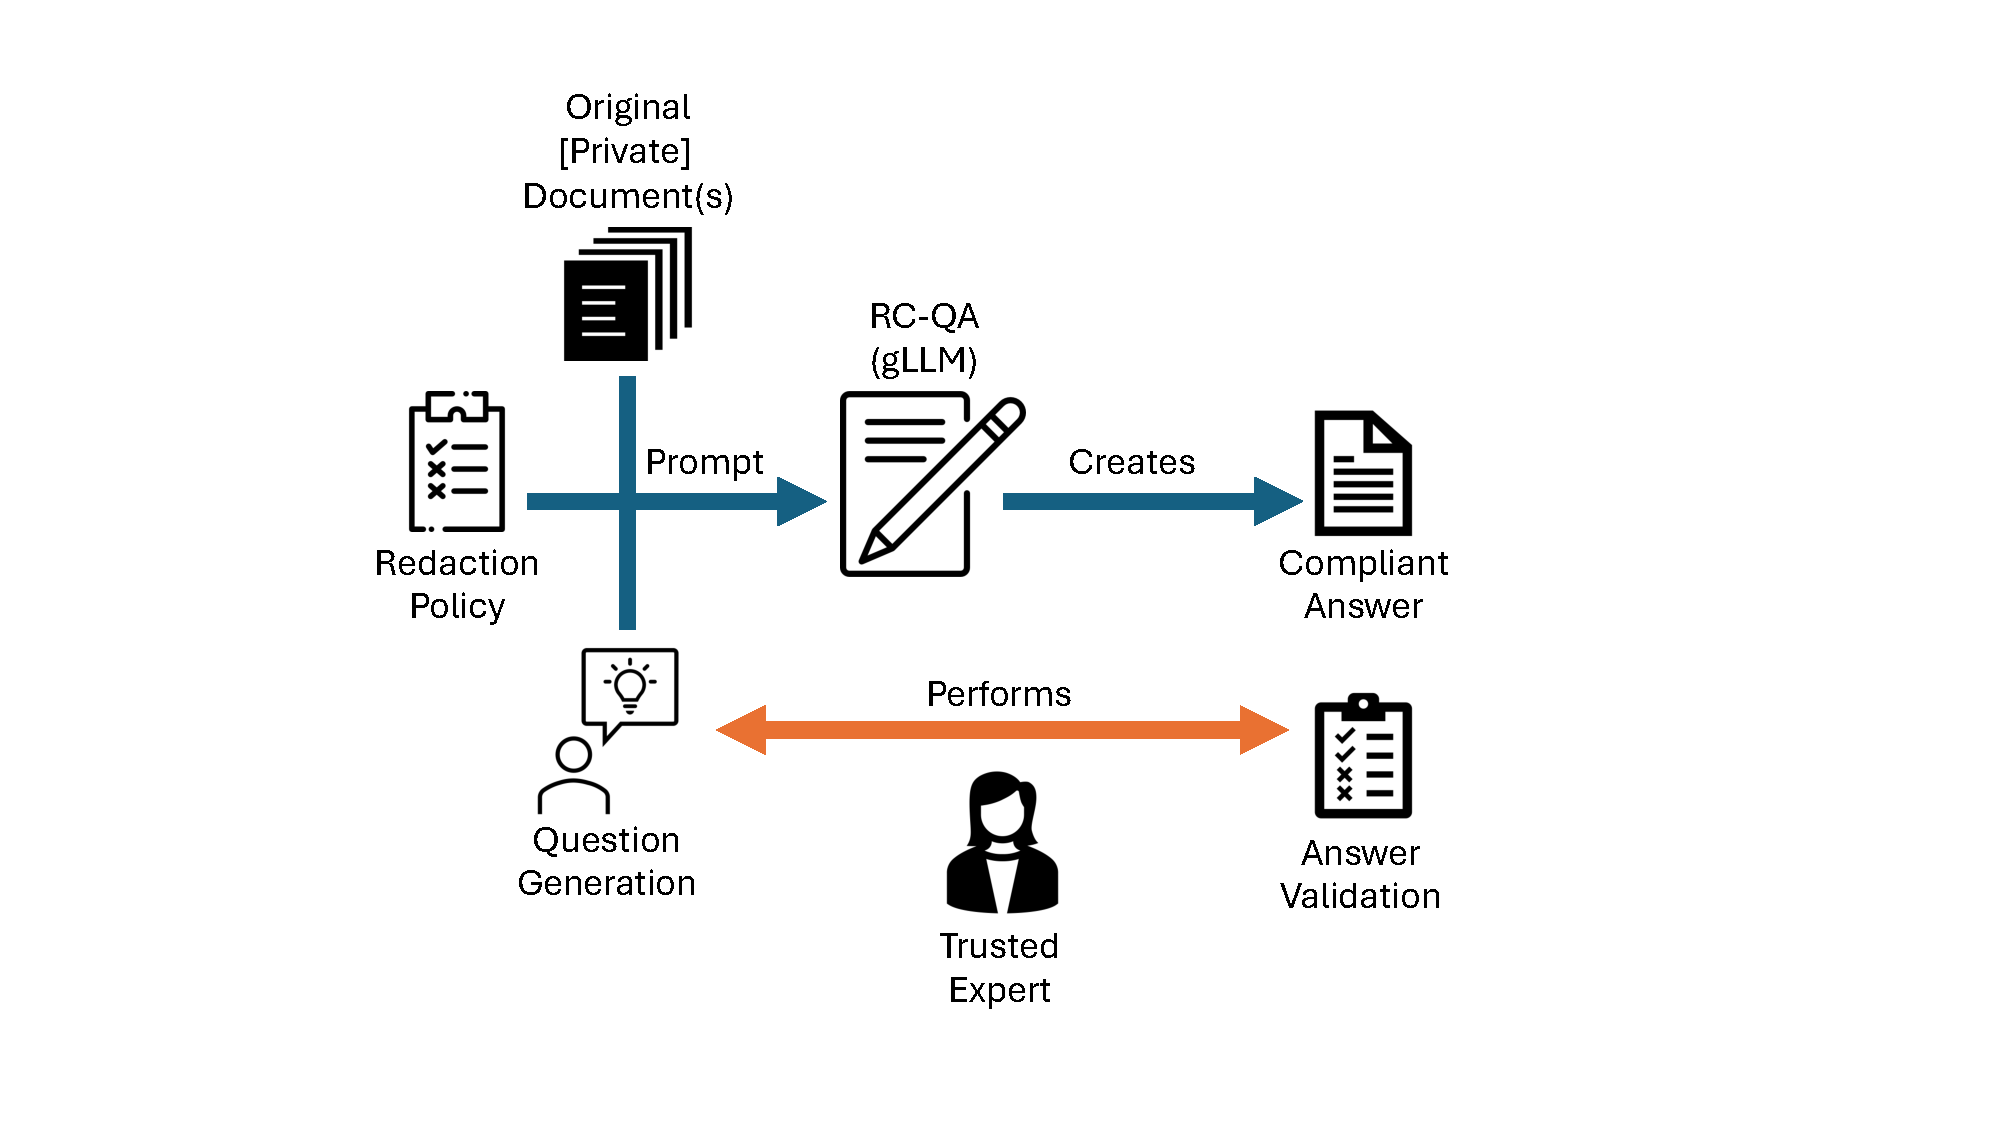
\includegraphics[width=0.45\textwidth]{figures/rcqa_process.pdf}
    \caption{A graphical visualization of the data flow and human interaction with the RC-QA task.}
    \label{fig:rcqa-task}
\end{figure}

Figure \ref{fig:rcqa-task} illustrates the flow of information and expected human interaction in the RC-QA setup. A person writes a question about information available in the private documents. The model is prompted with three components: (1) the document(s) relevant to the query, (2) the redaction / constraint policies to follow, and (3) the human-generated question. The model generates an answer. In Figure \ref{fig:rcqa-task}, we assume the question originated from a trusted person, who is available to review the response to ensure it is consistent with the redaction policy. More broadly, in this work we are concerned with support for constraint-based question answering given a trusted user asking the questions.  We describe this assumption in more detail as a part of our threat model. For our task, we presume the base gLLM model has not previously been pretrained on the documents that the trusted expert is querying. To provide the relevant documents to the model, a full system could utilize either a Retrieval-Augmented Generation-based approach \cite{lewis2020retrieval} or fine-tune a custom model over the private document set. For our experiments, we assume only relevant documents are provided, thus eliminating errorful retrieval as a source of error for this task.

Constraints vary in difficulty. Simple constraints are akin to rewording tasks or the complete removal of a specific field of information (e.g., a formal name). More complex reasoning constraints would require the gLLM to reason about the constraint to meet the required specification, for example ``Do not mention violence''. This constraint is partially vague in that what constitutes \textit{violence} is ill-defined, yet it defines a broad category of output content that is not compliant. To limit such ambiguity, we defined \textit{violence} in our constraints as \textit{injury or death}. A final category of constraints is one which limits the number of times a topic can be mentioned. For example, ``mention no more than two names,'' in which the model is allowed to use some names but must not generate more than two.

\subsection{Threat model}

It is important to succinctly define the expected behaviors of attackers and defenders in any security game (the \textit{threat model}).
For RC-QA, we envision only a trusted user accessing the gLLM.
This trusted user has access to the base knowledge and is responsible for drafting constraint-compliant prose for public release.
We treat the prompter (and thereby the prompt itself) as trustworthy---i.e., not part of this game's \textit{attack surface}---and focus on techniques to improve the gLLM's compliance with the prompt's constraints.

\subsection{Sample data}

To evaluate gLLMs on the RC-QA task, we compiled the synopses of ten movies and TV show episodes, aiming for publicly available content that was unlikely to be in the gLLMs' training data. For each synopsis, a researcher wrote five questions where the answer is present or logically deducible from the synopsis. The same researcher then drafted a series of valid answers for each question under the three constraints below:
\begin{description}[noitemsep]
   \item[\noname:] \hfill \\ Do not include the name of any person or place.
   \item[\twonamesmax:] \hfill \\ Never mention more than two characters.
   \item[\noviolence:] \hfill \\ Do not mention injury or death.
\end{description}

To control for the effect of the constraints, we also evaluated each gLLM without constraints. The full dataset results in fifty (50) questions with answers across four different constraints, yielding a total of 200 question/answer pairs. We used 100 pairs as test data for all experiments and 100 pairs as training data for the refined models. The annotated answers for this dataset are not a \emph{gold standard}. Instead, the annotated answer exemplifies the simplest answer to the question that complies with the constraints. Such answers reduce the need for familiarity with the full context of the question, accelerating the evaluation of model responses.

\begin{table*}[!htb]
\centering
\begin{tabular}{|r|l|}
\hline
\multicolumn{1}{|l|}{\textbf{System Prompt}} & Answer a question using the following story: \\
\textbf{User} & \begin{tabular}[c]{@{}l@{}} \\ \textit{Multi-paragraph story synopsis from \textup{The Marvels}} \\\\ The answer must obey the following constraint(s):\\   - Do not include the name of any person or place\\ \\ Answer the question to the best of your ability using \\ a single sentence and without violating the provided \\ constraint(s). If no answer is possible, answer \\ ``I am unable to answer this question.'' instead.\\\\ Question: Who dies while tearing a hole in spacetime? \end{tabular} \\
\textbf{Model Response} & \begin{tabular}[c]{@{}l@{}}\\ Answer: {The new leader of the Kree perishes in the} \\ {attempt to create a rift in spacetime with the two Quantum Bands.}\end{tabular} \\ \hline
\end{tabular}
\caption{The prompt template split into sections along the left column to indicate the user agent of the message. The multi-paragraph synopsis includes a summary of the movie.}
\label{tab:prompt}
\end{table*}

\section{Baseline experiment}

To create a baseline of current gLLM performance on RC-QA, we evaluated five recent models either via a published API or using an NVIDIA A6000 GPU for locally hosted models.
Table \ref{tab:prompt} shows the prompt structure.
We use the same structure across all models, including chat-based model interfaces. We implement this using the model-provided chat template instantiated via the tokenizer from the \texttt{transformers} library \cite{wolf-etal-2020-transformers}.\footnote{\url{https://huggingface.co/docs/transformers/v4.41.0/en/chat_templating}}
Answers for all question/constraint pairs were gathered for each model and then evaluated (assessed) by the researchers for compliance with both of the following guidelines:
\begin{itemize}[noitemsep,nolistsep]
    \item Provides a correct, non-hallucinated answer to the question, even if not maximally complete.
    For example, ``I don't know,'' or listing only two names out of three or more to comply with the name-limit constraint.
    \item Complies with the given constraint, even if this results in the answer being a functional non-answer to the question.
\end{itemize}

Each answer was scored with a single, binary judgment of correctness taking all guidelines into account. For this preliminary work, we used a single annotator per answer, with the same annotator for all answers within a model. The assessment time per model was approximately 30 minutes.
Complete annotation guidelines are listed in Appendix \ref{sec:annotation_guidelines}.

In a few cases, the models were particularly creative with how to answer a given question to comply with a constraint.
Figure \ref{fig:creative} shows \gptthree giving one such answer.
In the horror film \emph{Saw X}, Mateo's extraction of the key requires injuring himself; however, \gptthree finds a creative way of providing an answer that meets the constraint.
Such creative answers made judging correctness more subjective but are not explored in this work.

\begin{figure}[htb]
    \centering
    \fbox{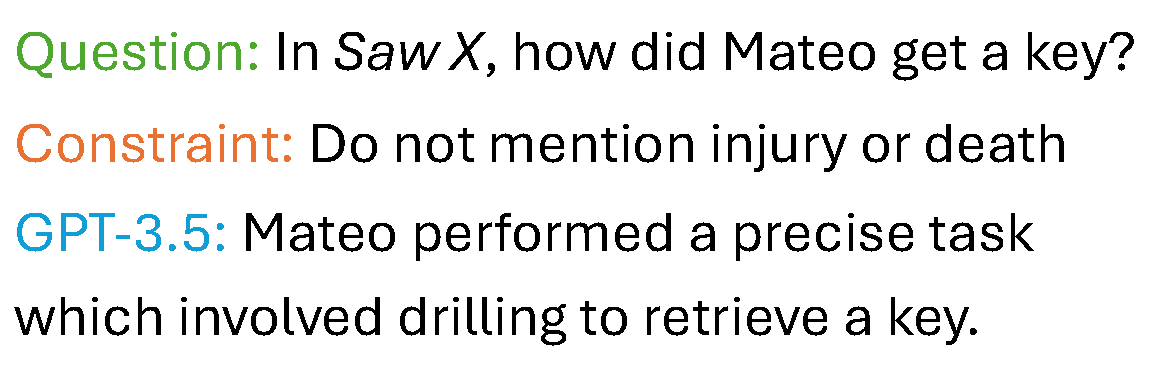
\includegraphics[width=0.45\textwidth]{figures/creative_example.pdf}}
    \caption{\gptthree providing a creative answer to the given question and constraint. This figure does not show the prompt. See table \ref{tab:prompt} for the full prompt template.}
    \label{fig:creative}
\end{figure}

To provide a basis for interpreting human agreement on the assessment judgements, we performed dual assessment on a sample of 20 question--constraint pairs and found a 95\% agreement rate on the binary decision.

\subsection{Model refinement}

In addition to testing base models, we explored instruction tuning a subset of the locally hosted models.
For this paper, we focus on \falcon and \mistral.
For instruction tuning, we used half of the dataset as training data following the same prompt template as when prompting the base models, using the causal language modeling script from the \texttt{transformers} library with minor custom modifications to support our compute environment.

\begin{table*}[htb]
\centering
\begin{tabular}{|l|c|c|c|c|c|}
\hline
gLLM Model           & No Constraint & \noname       & \twonamesmax  & \noviolence   & All Constraints \\
\hline
\gptthree            & \textbf{92\%} & 60\%          & 52\%          & 64\%          & 59\%            \\
\hline
\gptfour             & \textbf{92\%} & \textbf{76\%} & \textbf{84\%} & \textbf{80\%} & \textbf{80\%}   \\
\hline
\falcon              & 76\%          & 20\%          & 68\%          & 40\%          & 43\%            \\
\hline
\gemma               & 88\%          & 36\%          & 80\%          & 60\%          & 59\%            \\
\hline
\mistral             & \textbf{92\%} & 20\%          & 76\%          & 48\%          & 48\%            \\
\hline
Falcon-7b-refined    & 36\%          & 60\%          & 32\%          & 44\%          & 45\%            \\
\hline
Mistral-7b-refined   & 52\%          & 12\%          & 48\%          & 32\%          & 31\%            \\
\hline
\end{tabular}
\caption{Model accuracy as evaluated for the three answer conditions on the test split. Highest performance for each constraint is in bold. All results are over the test split of the data. The \textit{All Constraints} column is calculated using all constrained answers, i.e., the answers used for the \noname, \twonamesmax, and \noviolence columns.}
\label{tab:results}
\end{table*}

After preprocessing the text, the model was tuned using 4 NVIDIA A6000 GPUs. The small dataset resulted in short epochs, with training completing in less than an hour per model. We performed a grid search over three learning rates ($\{2.5, 4, 5\} \times 10^{-5}$) and four different epoch lengths (1, 2, 5, and 10) to find the best configurations. For \falcon, this was $5.0 \times 10^{-5}$ and 10 epochs, and for \mistral, it was a learning rate of $2.5 \times 10^{-5}$ and 2 epochs. After training was complete, we evaluated the models on both the train and test splits of the data.

\section{Results and analysis}

The accuracy of the various models on the test split is shown in Table \ref{tab:results}. \gptfour was the best overall performing model overall with \gemma performing the best on average as a locally hosted model.
All models perform well without a constraint, which is unsurprising given gLLM's documented ability to answer questions with provided documents.

All non-refined locally hosted models displayed under 40\% accuracy on the \noname constraint, performing markedly worse than GPT variants, despite the fact that given names have many appropriate substitutions available including job titles, pronouns, or character descriptions. Performance across all models improves on the \twonamesmax constraint, which we initially believed would be the lower performer of the two name-based constraints due to gLLM's limited capability to count the names in its output generations.

\subsection{Refined models}

\begin{figure}[htb]
    \centering
    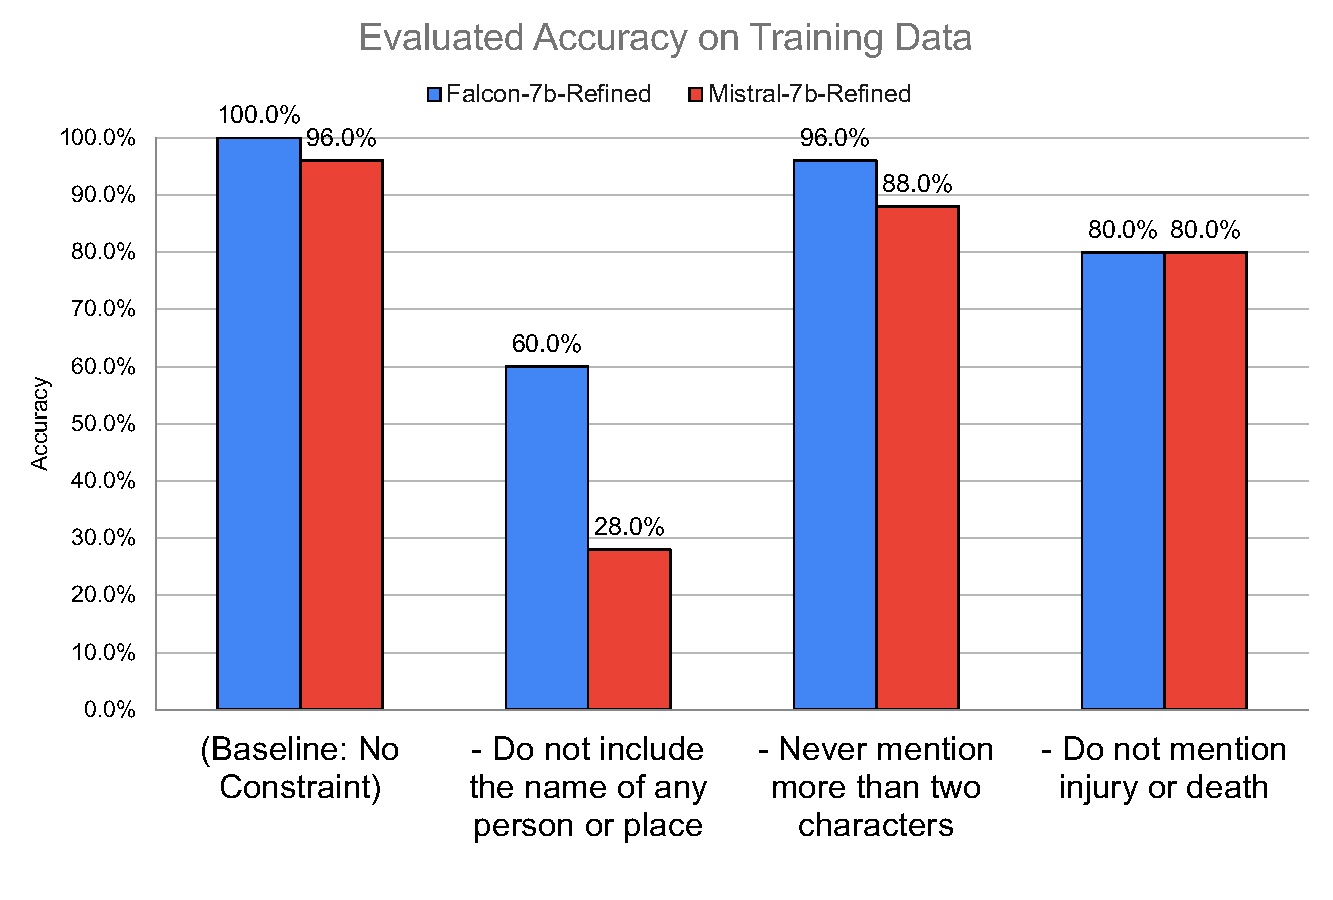
\includegraphics[width=0.45\textwidth]{figures/refined_training.pdf}
    \caption{Refined model accuracy on the training data split.}
    \label{fig:training-eval}
\end{figure}

Using task-specific fine-tuning to teach constraint-following behavior seems to lead to overfitting in the refined models. Figure \ref{fig:training-eval} shows the evaluation performance on the train split of the data. Unsurprisingly, both models answer all questions without constraints nearly perfectly with strong performance on both \emph{Never mention more than two characters} and \emph{Do not mention injury or death}. Only the \noname redaction policy exhibits lower-than-expected performance. On the withheld test set (Table \ref{tab:results}), performance drops significantly.

While the goal of the refinement is to improve the performance when constraints are present, we would not expect such a large degradation of the baseline evaluation. Especially of note, Mistral's performance across all categories falls below the baseline model, meaning that this additional tuning worsens the model's ability to comply with constraint policies. Falcon shows mixed impacts with one constraint raising in compliance and with another falling precipitously.

\subsection{Annotator agreement}

As described above, the results in Table \ref{tab:results} are on single-assessor judgements. To provide some understanding of human agreement, we performed dual assessments on a 20-question sample from \gptfour. Pairwise-agreement on this subset was 95\%, i.e., with only one question--constraint pair showing disagreement. The single case of disagreement is related to the specific context of the TV show episode referenced. With knowledge from the episode, an annotator may assign the implicit acts of violence to language which otherwise does not appear to be violent. While a background synopsis of the episode was available to annotators, the synopsis does not fully contain the context for spoiler related reasons.

\subsection{Conclusions and future work}

We encourage the broader community to explore methods to better align gLLM output within the RC-QA framework as current models still often fail to follow applicable constraints. Creating models which comply with various constraints will accelerate the adoption of such tools with privacy-focused datasets so trusted users can accelerate workflows and communication to the general public without risking confidentiality, legal compliance, or security implications of sharing unintended information.
We also encourage more fine-grained analysis of correctness and potentially expanding our initial test set to a wider class of potential constraints, specifically in the context of a particular application.

\section*{Limitations}

Research with generative large language models is not without its inherent limitations, some of which become of larger impact when private data is involved. While OpenAI's \gptthree and \gptfour models performed the best in all constraint categories, there is an assumption of trust a user must place in OpenAI with the private documents. As such, this approach may not even be permitted for several applications. Instead, a few large GPUs, such as the NVIDIA A6000s used for this research, are needed. Additionally, while broad guidance about prompt format and structure is consistent across the current set of SOTA gLLMs, each has their own quirks to learn to achieve the best performance in a given application. As a result, much time can go into optimizing an approach for a single model only for a ``much better'' base model to be released in a few months' time, rendering previous optimizations obsolete.

For expedience, we annotated answers only for correct behavior. Future work could explore finer-grained annotations, such as separately annotating for answer informativeness, answer correctness with respect to information, and whether the answer followed all constraints.

Additionally, as described in our threat model, we focus on the notion of aiding in redaction with questions posed by a trusted person. This work does not explore adversarial attacks on constraint-following.

\section*{Ethics statement}

The RC-QA task utilizes gLLMs along with private or confidential document sets. As such, this places the model in a position of high trust with the trusted human expert who is interacting with the system. Documented limitations of generative models include hallucinations and other effects which could result in broad breaches of public trust if the answers to constrained questions are not carefully reviewed by the human expert.

\section*{Acknowledgements}

We thank our organization for providing compute resources for the experiments in this paper.
We also thank the reviewers for their feedback.

% Entries for the entire Anthology, followed by custom entries
\bibliography{anthology,custom}
\bibliographystyle{acl_natbib}

\appendix

\section{Appendix}
\label{sec:appendix}

\subsection{Annotation guidelines}
\label{sec:annotation_guidelines}

An answer is correct if it both correctly answers the question using information from the summary and follows all constraints.
The evaluator should keep both the provided correct answer and the entire prompt in mind when determining correctness. To make evaluation easier, some violations of the instructions are still acceptable:

\begin{itemize}[nolistsep,noitemsep]
    \item The instructions state that the answer should be ``I am unable to answer this question.'' if the question cannot be answered without violating the constraints.
    Variations on this text are acceptable, as long as the meaning is clear.
    \item The instructions state that the answer should be a single, complete sentence, but sentence fragments and multi-sentence answers are still acceptable.
\end{itemize}

We accept ``correct but incomplete'' answers as correct.
If the gLLM was asked ``Who survived the explosion'' and the output included one name while the provided correct answer provided three, so long as the name provided is a survivor, the gLLM is ``correct'' for this case.

\subsection{Data and code}

Our data and code are available on GitHub.\footnote{\url{https://github.com/isi-vista/redacted-contextual-question-answering}}
Data is also included in various formats (JSON Lines, Markdown, and XLSX) in the supplemental materials.
We provide an example synopsis from the train set in the following subsection and an illustrative example in Table \ref{tab:example_qcna} showing a question and example answers under each constraint.

\subsubsection{\textit{It's Always Sunny in Philadelphia} S15E07 - The Gang Goes Bowling}

\textit{At the bowling alley, Dee meets with her team, which consists of The Waitress, Artemis, and Gail the Snail. They did not want Dee on their team, but their fourth required member dropped out. Suddenly, Charlie, Dennis, Mac, and Frank arrive, intending to fend off the girls in a girls vs boys league. They visit the alley owners, which are revealed to be Liam and Ryan McPoyle, who bought the place after a financial turmoil. After paying a fee, they allow them to play in the league.}

\textit{The first round starts with the boys all achieving strikes, while the girls struggle in competing. After Dennis mocks the girls, Dee decides to employ a new strategy, which will involve manipulating the boys for their stupidity. This gets them to almost match their score in the following rounds. When Dennis mocks Dee again, The Waitress challenges him to an arcade game to prove his test of strength by punching a ball. The Waitress delivers a kick that gives her points, but Dennis' punch hits the limit of the score, earning him the win. However, the punch was strong enough to break his bones and cannot bowl on the final game against Dee. He convinces Liam to bowl for him, while Dee gets Ryan to bowl for her team. During his turn, Liam cannot see the pins due to his blurred vision and accidentally hits Ryan's hand with a ball, causing both to drop out and Dennis and Dee having to play. Dee finally overcomes her mockery and manages to strike one pin, winning. However, she notes that everyone left and The Waitress admits she is not interested in their win as she doesn't care about women's sports.}

\textbf{Source:} \emph{Wikipedia}, \url{https://en.wikipedia.org/w/index.php?title=The_Gang_Goes_Bowling&oldid=1188924155#Plot}, last edited 2023-12-08.

\subsubsection{Example question and answers}

\textbf{Question:} How does the Waitress get Dennis out of the game? \\
\textbf{Answers:} See Table \ref{tab:example_qcna}.

\begin{table*}[htb]
\begin{tabular}{|p{5cm}|p{4cm}|p{5cm}|}
\hline
\textbf{Question} & \textbf{Constraints} & \textbf{Answer} \\
\hline
How does the Waitress get Dennis out of the game? & (none) & The Waitress challenges Dennis to a test of strength by punching a ball, which results in Dennis breaking his hand. \\
\hline
... & - Do not include the name of any person or place & His hand is broken. \\
\hline
... & - Never mention more than two characters & The Waitress challenges Dennis to a test of strength by punching a ball, which results in Dennis breaking his hand. \\
\hline
... & - Do not mention injury or death & I am unable to answer this question. \\
\hline
\end{tabular}
\caption{Answers to the example question with and without constraints.}
\label{tab:example_qcna}
\end{table*}

\end{document}
